\documentclass[tikz,fontsize=8pt]{standalone}
\usepackage{fourier}
\usetikzlibrary{arrows.meta}
\usetikzlibrary{calc}
\tikzset{>=latex}
\definecolor{bookblue}{RGB}{0,173,239}
\definecolor{bookpink}{RGB}{236,0,140}
\definecolor{bookgreen}{RGB}{50,200,0}
\definecolor{bookbluearea}{RGB}{204,239,252}
\tikzstyle{blueline}=[draw=bookblue,line width=0.2mm]
\tikzstyle{pinkline}=[draw=bookpink,line width=0.2mm]
\tikzstyle{greenline}=[draw=bookgreen,line width=0.2mm]
\tikzstyle{blackline}=[draw=black,line width=0.2mm]
\tikzstyle{bluearea}=[fill=bookbluearea]

\usepackage{scrextend}
\changefontsizes[8pt]{8pt}
\usetikzlibrary{decorations.pathreplacing}
\begin{document}
  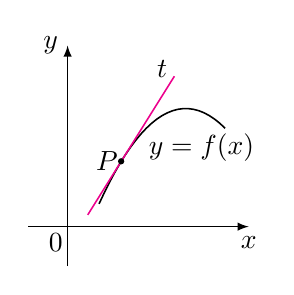
\begin{tikzpicture}
    \node at (-0.15,-0.2) {0};
    \draw[->] (-0.5,0) -- (2.3,0) node[below] {$x$};
    \draw[->] (0,-0.5) -- (0,2.3) node[left] {$y$};
    
    \draw[blackline,domain=-1.1:0.5] plot (\x+1.5,{-(\x)^2+1.5});
    \draw[pinkline] (0.256,0.15) -- (1.356,1.91);
    \fill (0.68,0.83) circle (0.4mm);
    \node at (0.5,0.83) {$P$};
    \node at (1.2,2) {$t$};
    \node at (1.7,1) {$y=f(x)$};
  \end{tikzpicture}
\end{document}